\documentclass[titlepage, a4paper, 11pt, reqno, openany]{report}
%a4paper leqno reqno letterpaper  a5paper b5paper executivepaper legalpaper
%ladscape twocolumn oneside twoside
%titlepage openany
%article report book slides proc minimal
%
\usepackage{amsfonts}
%\usepackage[brazil]{babel} %linguagem do documento
%\usepackage{babel}
\usepackage[portuguese]{babel}
\usepackage{babelbib}
%\usepackage[utf8]{inputenc} %reconhece acento e cedilha
\usepackage{amssymb}
\usepackage{latexsym}
\usepackage{amsmath}
%\usepackage[fleqn]{amsmath}
%\usepackage{mathtools}
%\usepackage[fleqn]{mathtools}
\usepackage{pxfonts} %permite simbolos matemáticos
\usepackage{mathrsfs} %permite uso de fontes para conjuntos
\usepackage[normalem]{ulem} %permite sublinhar palavras
\usepackage{mathrsfs} %permite o uso de letras trabalhadas
%\usepackage[margin=1in, paperwidth=8.5in, paperheight=11in]{geometry}
%\usepackage[top=1in, bottom=1in, left=1in, right=1in]{geometry}
%\usepackage{fullpage}
\usepackage[top=1.5cm,left=1.5cm,right=1.5cm,bottom=1.5cm]{geometry} %margens
\usepackage{graphicx} %permite inserir figuras
\usepackage[usenames]{color} %permite letras coloridas
\usepackage{makeidx} %pra criar índice remissivo
%\usepackage{tikz}
%\usepackage{pgfplots}
\usepackage{mathptmx}
%\usepackage{named}
\usepackage{enumerate}
%\usepackage{amscls}
%alguns pacotes nao sao reconhecidos, ter atencao quais usar em differents computadores.
\usepackage{float}
\usepackage{caption}
\usepackage{verbatim}
%%%%%%%%%%%%%%%%%%%%
\newtheorem{theorem}{Theorem}
\newtheorem{lemma}{Lemma}
\newtheorem{definition}{Defini\c{c}\~{a}o}
\newtheorem{notation}{Notation}
%%%%%%%%%%%%%%%%%%%%

\bibliographystyle{babplain}

\makeindex

%
\begin{document}
\begin{titlepage}
\begin{minipage}{0.95\linewidth}
\centering

\includegraphics[scale=0.60]{./image/ISEP_marca_cor_grande.png}
\label{Capa}
\title{Electr\'{o}nica de Pot\^{e}ncia}
\author{\emph{S\'{e}rgio Santos},\;$N^o$:\; 1020881}
\date{\today}
\maketitle
\end{minipage}
\end{titlepage}
%titlepage
%
\tableofcontents
%
\appendix
%
\pagestyle{plain}%plain headings empty
%
%few lessons \newline \newpage only in text.
%\pagestyle{headings} %estilo de numeração
%{\tiny text}{\scriptsize text}{\footnotesize text}{\small text}{\normalize text}{\large text}{\Large text}{\huge text}{Huge text}{\it text}{\bf text}{\tt text}\underline{text}
%\newline \newpage \linebreak \\[distance]
%\. \, \; quad qquad hspace{xx cm} vspace{xx cm}
%{\color{cor}text}
%\footcite{•}\twocolumn\onecolumn
% $ formula $ $$ formula $$ \nonumber \\
%\frac{•}{•} \dfrac{•}{•} \sqrt[•]{•} \binom{}{}
%\mathbb{NZqRC} \mathcal{texto} \mathfrak{texto}
%\vert \Vert \leq \geq \neq \to \lim
%displaystyle \int \sum \prod \cup \cap
%\longleftarrow \overline{•} \langle
%\hline \caption \label \centering \ref{Capa}
%%%%%%%%%%%%%%%%%%%%%%%%%%%%%%%%%%%%%%%%%%%
%
\part{Problema 2 - A1}\label{part1}
\section{Corrente Alternada circuito $RLE$ com interruptor.}
%
\begin{flushleft}
Considere o circuito da Figura \ref{grafico 1} Suponha $V_s$ = tens\~{a}o da rede el\'{e}ctrica nacional ($240V\,\, 50Hz$).\par
\end{flushleft}
%
\begin{enumerate}
%1
\item
O interruptor \'{e} fechado em $t=0$, quando a fase da sinusoide apresenta o \^{a}ngulo $\alpha$. ($\alpha$ \'{e} tamb\'{e}m conhecido como \^{a}ngulo de disparo, nomeadamente quando se utiliza um tir\'{i}stor no lugar do interruptor).\par
%
\begin{figure}[H]
\centering
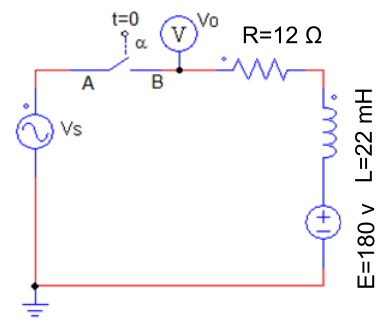
\includegraphics[scale=0.75]{./image/Screenshot21.png}\\
\caption{Circuito $RLE$ comutado}
\label{grafico 1}
\end{figure}\par
%
\begin{enumerate}
%1a
\item 
Deduza as express\~{o}es gen\'{e}ricas*(1) para $V_R(\omega t)$, $V_L(\omega t)$ e $I_o(\omega t)$, especificando as componentes no regime transit\'{o}rio $(i_n(\omega t))$ e permanente $(i_p(\omega t))$.\par Equa\c{c}\~{a}o do circuito :\par
\begin{equation}
\boxed{ V_{m\acute{a}x}\ \sin(\omega t + \alpha)=R\ i(t)+L\ \frac{d i(t)}{dt}+E }
\end{equation}\par
%
Sabendo que,\par
\begin{equation}
i(t)=C_T\ e^{-\frac{R}{L}t}+\frac{V_{m\acute{a}x}}{\overline{Z}}\sin(\omega t + \alpha - \phi_p)-\frac{E}{R}
\end{equation}\par
%
mas queremos que as fun\c{c}\~{o}es  deduzidas sejam dependente de {\color{red}$\omega t$} temos que recorrer a mudan\c{c}a de vari\'{a}vel \par
%
\begin{equation}
I(\omega t)= \overbrace{C_T\ e^{-\frac{R}{L \omega}\omega t}}^{i_n(\omega t)} + \overbrace{\frac{V_{m\acute{a}x}}{\overline{Z}}\sin(\omega t + \alpha - \phi_p)-\frac{E}{R}}^{i_p(\omega t)}
\end{equation}\par
%\overset{overset}{expresssion} \not= \sideset{left}{right}
tomamos em conta que as condi\c{c}\~{o}es iniciais s\~{a}o nulas, isto \'{e}, $I_{0^-}=0$, que \'{e} o mesmo que $\omega t = 0$.\par
%
\begin{eqnarray}
C_T &=& \frac{E}{R}-\frac{V_{m\acute{a}x}}{\overline{Z}}\sin(\alpha - \phi) \\
\phi_p &=& \arctan \left( \frac{\omega L}{R} \right)
\end{eqnarray}\par
%
tamb\'{e}m\par
%
\begin{equation}
C_T = \frac{V_{m\acute{a}x}}{R^2 + (\omega L)^2}(L \omega \cos(\alpha) - R \sin (\alpha))+\frac{E}{R}
\end{equation}\par
%
logo,\par
\begin{eqnarray}
V_R(\omega t) &=& R \times I_o(\omega t)\\
V_L(\omega t) &=& L \; \frac{d\, I_o(\omega t)}{d\omega t} \times \omega \\
 &=& \frac{\omega \; L \; V_{m\acute{a}x}}{\overline{Z}} \; \cos(\omega t + \alpha - \phi_p) - R \; C_T \; e^{\frac{-R}{\omega L} \, \omega t} \nonumber \\
I_o(\omega t) &=& C_T\ e^{-\frac{R}{L \omega}\omega t}+\frac{V_{m\acute{a}x}}{\overline{Z}}\sin(\omega t + \alpha - \phi)-\frac{E}{R}\\
i_n(\omega t) &=& C_T\ e^{-\frac{R}{L \omega}\omega t}\\
i_p(\omega t) &=& \frac{V_{m\acute{a}x}}{\overline{Z}}\sin(\omega t + \alpha - \phi_p)-\frac{E}{R}\\
\end{eqnarray}\par
%1b
\item 
Determine a constante de tempo do circuito ($\tau$).\\
$\tau=\frac{L}{R}=\frac{22\times 10^-3}{12}\approx 0.001833^.\, sec$,\\
e o seu per\'{i}odo da fonte sinusoidal, $T_o=\frac{1}{f}=\frac{1}{50}=0.02\, sec$
%1c
\item 
Supondo que o interruptor \'{e} fechado $6ms$ ap\'{o}s o in\'{i}cio da sinus\'{o}ide, determine 
o \^{a}ngulo de disparo $\alpha$;\\
$\alpha = \omega \times 6\times 10^-3\,\, rad$\\
$\alpha = 108^o$
%1d
\item
Para o \^{a}ngulo $\alpha$ determinado em c) e socorrendo-se do {\bf Excel} (ou equivalente, {\bf Open Office}), obtenha um gr\'{a}fico que inclua as formas de onda de $V_s(\omega t)$, $V_R(\omega t)$, $V_L(\omega t)$ e $E$, e um outro gr\' {a}fico com a forma de onda de $I_o(\omega t)$, e com as componentes no regime transit\'{o}rio $(i_n(\omega t))$ e permanente $(i_p(\omega t))$.\par
%
\begin{equation}
V_s(\omega t) = \frac{V_{m\acute{a}x}}{\overline{Z}} \; \sin(\omega t + \alpha); \quad
V_R(\omega t) = R \; I_o(\omega t); \quad
V_L(\omega t) = L \; \dfrac{d I_o(\omega t)}{d \omega t} \times \omega; \quad
E = 180 \nonumber
\end{equation}\par
%
\begin{figure}[H]
\centering
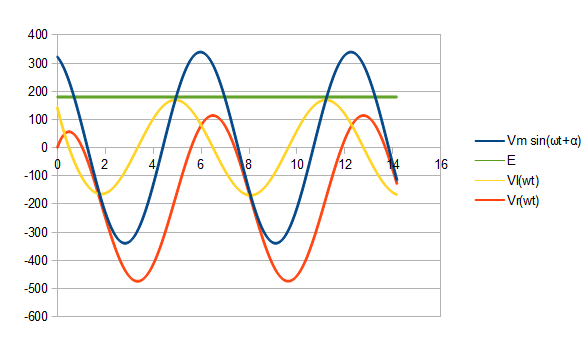
\includegraphics[width=0.90\linewidth]{./image/P2A1p1_1_d_1.png}
\caption{Tens\~{o}es}
\label{figura 2}
\end{figure}\par
%
\begin{figure}[H]
\centering
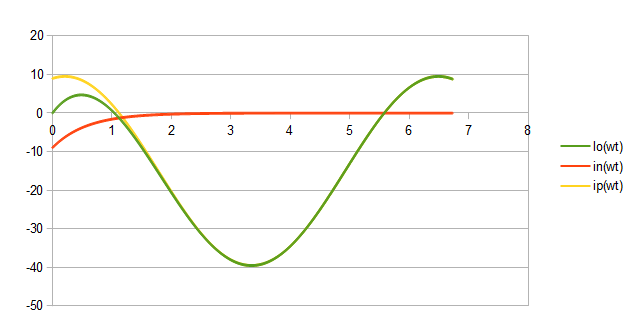
\includegraphics[width=0.90\linewidth]{./image/P2A1p1_1_d_2.png}
\caption{Correntes}
\label{figura 3}
\end{figure}\par
%
\end{enumerate}
%2
\item
Suponha agora que \underline{entre $A$ e $B$ \'{e} colocado um d\'{i}odo}, com o \^{a}nodo ligado a $A$, e ainda que \underline{$E=0$}.\par
%
\begin{enumerate}
%2a
\item
Socorrendo-se do {\bf Excel} determine o tempo de condu\c{c}\~{a}o $t_c$ do d\'{i}odo; e o \^{a}ngulo correspondente de condu\c{c}\~{a}o $\gamma$; \\[0.2cm]
%
O d\'{i}odo esta em condu\c{c}\~{a}o pelos valores aproximados da tabela do {\bf LibreOffice} nos intervalos de $\omega t = 0 \; rad$ at\'{e} $\omega t \approx 1,7303419 \; rad$ e de $\omega t \approx 4,39946745
 \; rad$ at\'{e} $\omega t = 2 \pi \; rad$ \par
Portanto este conduz no total $\omega t \approx 3,614059757 \; rad$ que da o total de $\gamma \approx 207,070371^o$ (graus) em condu\c{c}\~{a}o durante um periodo. \par
Como $\omega t \approx 3,614 \; rad$ o tempo de condu\c{c}\~{a}o $t_c = \frac{\omega t}{\omega}$, ou seja, $t_c = \frac{3,614}{2 \pi 50} \approx 11,50 ms$ \par
%2b
\item
Obtenha um gr\'{a}fico que inclua as formas de onda de $V_s(\omega t)$, $V_R(\omega t)$, $V_L(\omega t)$ e $E$, e outro gr\'{a}fico com a forma de onda de $I_o(\omega t)$ e com as componentes no regime transit\'{o}rio $(i_n(\omega t))$ e permanente $(i_p(\omega t))$.\\[0.2cm]
Condi\c{c}\~oes iniciais para $\omega t = 0 \; rad$ at\'{e} $\omega t \approx 1,7303419 \; rad$ \quad e \quad $\omega t \approx 4,39946745 \; rad$ at\'{e} $\omega t = 2 \pi \; rad$, \par
Sabendo que para condi\c{c}\~{o}es iniciais nulas, $i_p(0^-)=-i_n(0^-)$, e $\phi_n \approx 0,474$, isto \'{e} o avan\c{c}o da corrente transit\'{o}rio. \par
%
\begin{figure}[H]
\centering
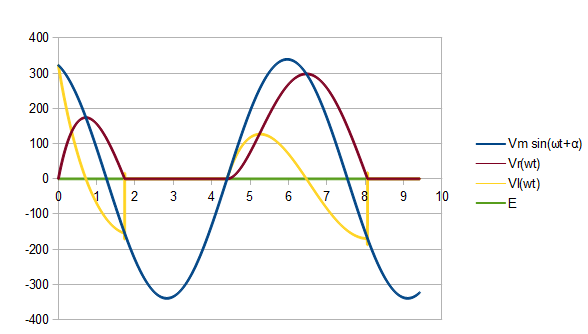
\includegraphics[width=0.90\linewidth]{./image/P2A1p1_2_a_1.png}\\
\caption{Tens\~{o}es}
\label{grafico 4}
\end{figure}\par
%
\begin{figure}[H]
\centering
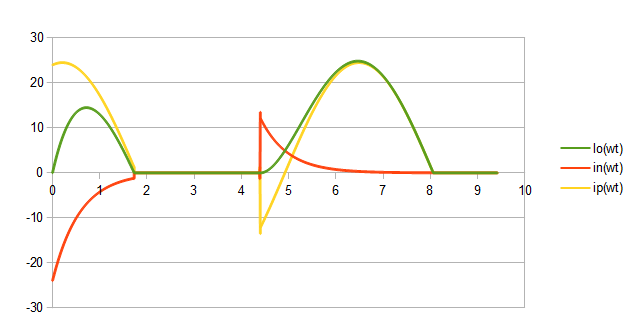
\includegraphics[width=0.90\linewidth]{./image/P2A1p1_2_a_2.png}\\
\caption{Correntes}
\label{grafico 5}
\end{figure}\par
%
%2c
\item
Calcule*(2) os valores m\'{e}dios da tens\~{a}o e da corrente na carga $V_{oAV}$ e $I_{oAV}$;\par
C\'{a}lculos efetuados utilizando a ferramenta {\bf wxMaxima}. \par
Intervalo $[0 \; ; \; 2\pi]$ \par
%
$\omega t = 0; \rightarrow \omega t \approx 1,730; \; \alpha \approx 1,885; $ \par
$\omega t = 4,399; \rightarrow \omega t = 2 \pi; \; \alpha \approx 1.885; $ \par
\begin{flalign}
V_{oAV}=&\frac{1}{2 \pi} \; \left( \int_0^{1,730} \sqrt{2} \;  240 \sin(\omega t + \alpha) \; d \omega t + \int_{4,399}^{2 \pi} \sqrt{2} \;  240 \sin(\omega t + \alpha) \; d \omega t \right) & \\
=&102.097 & \nonumber
\end{flalign}
$\omega t = 0; \rightarrow \omega t \approx 1,730; \; \alpha \approx 1,885; $ \par
$\omega t = 0; \rightarrow \omega t \approx 1,885; \; \alpha = 0; $ \par
\begin{flalign}
I_{oAV} =& \frac{1}{2 \pi} \; \left( \left. \int_0^{1,730} I_{o}(\omega t) \; d \omega t \right|_{\alpha = 1,885} + \left. \int_0^{1,885} I_{o}(\omega t) \; d \omega t \right|_{\alpha = 0}
\right) & \\
=& 6,266 & \nonumber
\end{flalign}
%2d
\item
Calcule*(2) os valores eficazes da tens\~{a}o e da corrente na carga $V_{oRMS}$ e $I_{oRMS}$;\par
Intervalo $[0 \; ; \; 2\pi]$ \par
%
$\omega t = 0; \rightarrow \omega t \approx 1,730; \; \alpha \approx 1,885; $ \par
$\omega t = 4,399; \rightarrow \omega t = 2 \pi; \; \alpha \approx 1.885; $ \par
\begin{flalign}
V_{oRMS}=&\sqrt{\frac{1}{2 \pi} \; \left( \int_0^{1,730} (\sqrt{2} \;  240 \sin(\omega t + \alpha))^2 \; d \omega t + \int_{4,399}^{2 \pi} (\sqrt{2} \;  240 \sin(\omega t + \alpha))^2 \; d \omega t \right)} & \\
=&171,523 & \nonumber
\end{flalign}
$\omega t = 0; \rightarrow \omega t \approx 1,730; \; \alpha \approx 1,885; $ \par
$\omega t = 0; \rightarrow \omega t \approx 1,885; \; \alpha = 0; $ \par
\begin{flalign}
I_{oRMS} =& \sqrt{\frac{1}{2 \pi} \; \left( \left. \int_0^{1,730} I^2_{o}(\omega t) \; d \omega t \right|_{\alpha = 1,885} + \left. \int_0^{1,885} I^2_{o}(\omega t) \; d \omega t \right|_{\alpha = 0}
\right)} & \\
=& 9,746 & \nonumber
\end{flalign}
%2e
\item
Calcule*(2) a pot\^{e}ncia entregue \`{a} carga $RLE$.\par
Intervalo $[0 \; ; \; 2\pi]$ \par
%
$\omega t = 0; \rightarrow \omega t \approx 1,730; \; \alpha \approx 1,885; $ \par
$\omega t = 0; \rightarrow \omega t \approx 1,885; \; \alpha = 0; $ \par
%
\begin{flalign}
P_{oAV} =& \frac{1}{2 \pi} \; \left( \left. \int_0^{1,730} V_o(\omega t) \; I_{o}(\omega t) \; d \omega t \right|_{\alpha = 1,885} + \left. \int_0^{1,885} V_o(\omega t) \; I_{o}(\omega t) \; d \omega t \right|_{\alpha = 0}
\right) & \\
P_{o1} =& 4286.89493572789  & \nonumber \\
P_{o2} =& 5125.162040769396 & \nonumber \\
P_{o} =& 9412.056976497286 & \nonumber \\
P_{oAV} =& 1497.975392472102 & \nonumber
\end{flalign}
%
\end{enumerate}
\end{enumerate}
%
\begin{abstract}
Foi deduzido as express\~{a}o matem\'{a}ticas complexas como demonstra a Parte \ref{eq}, tamb\'{e}m foi feito uma analise rigorosa recorrendo ao {\bf LibreOffice} obtendo as formas de ondas, observando seu comportamento quanto aos desfazamentos e condu\c{c}\~{a}o, e os valores calculados s\~{a}o pr\'{o}ximos dos obtidos pelo simulador {\bf PSIM}.
\end{abstract}
%
\appendix
%%%%%%%%%P2A2%%%%%%%%%%
\part{Problema 2 - A2} \label{P2A2}
\section{Corrente Alternada circuito $RLE$ com tir\'{i}stor.}

\begin{enumerate}
%1
\item
Recorrendo ao {\bf PSIM}, confirme todas as formas de onda e valores obtidos na Parte \ref{part1} \par
%
1d) \par
\begin{figure}[H]
\centering
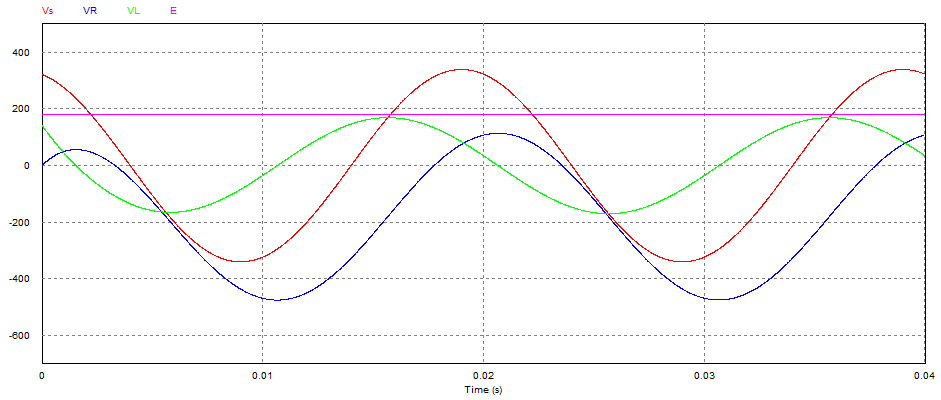
\includegraphics[width=0.90\linewidth]{./image/PSIMP2_1_1.png}\\
\caption{Tens\~{o}es}
\label{grafico 6}
\end{figure}\par
%
\begin{figure}[H]
\centering
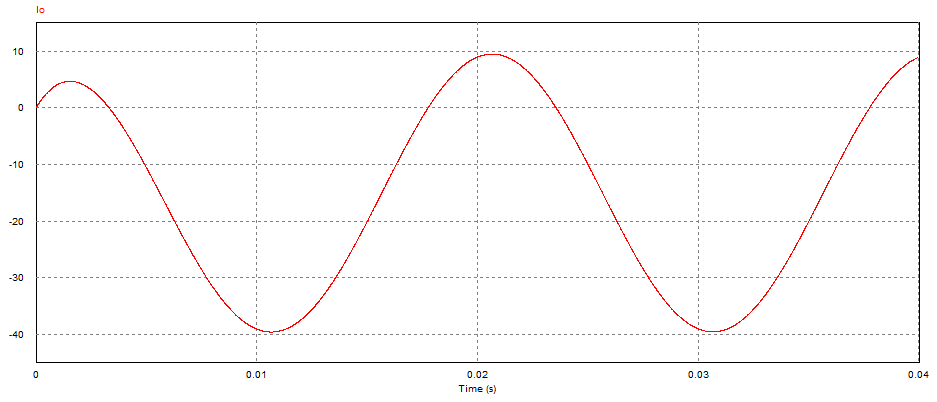
\includegraphics[width=0.90\linewidth]{./image/PSIMP2_1_2.png}\\
\caption{Corrente}
\label{grafico 7}
\end{figure}\par
%
2b)
%
\begin{figure}[H]
\centering
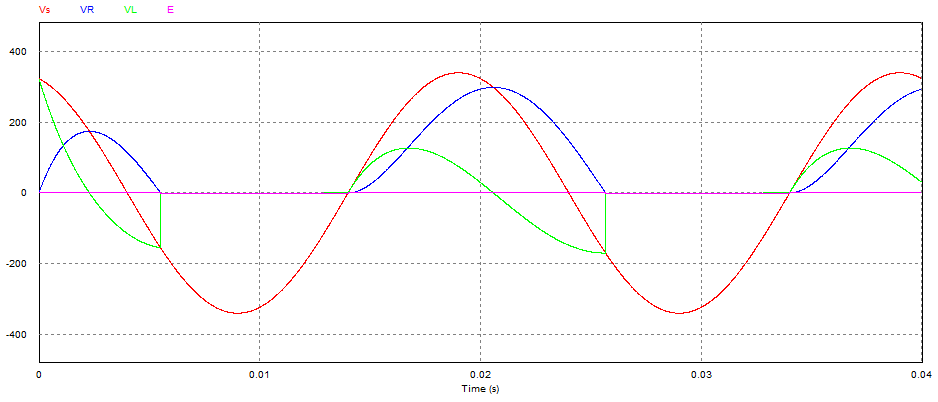
\includegraphics[width=0.90\linewidth]{./image/PSIMP2_1_3.png}\\
\caption{Tens\~{o}es}
\label{grafico 8}
\end{figure}\par
%
\begin{figure}[H]
\centering
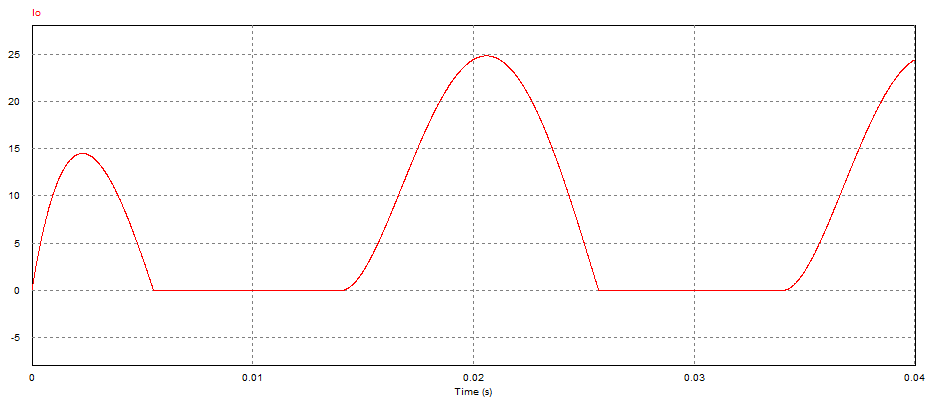
\includegraphics[width=0.90\linewidth]{./image/PSIMP2_1_4.png}\\
\caption{Corrente}
\label{grafico 9}
\end{figure}\par
%
Considere agora o circuito da Figura \ref{grafico 10} Suponha $Vs$ = tens\~{a}o da rede el\'{e}ctrica nacional. O tir\'{i}stor \'{e} disparado para o \^{a}ngulo $\alpha$.\par
%
\begin{figure}[H]
\centering
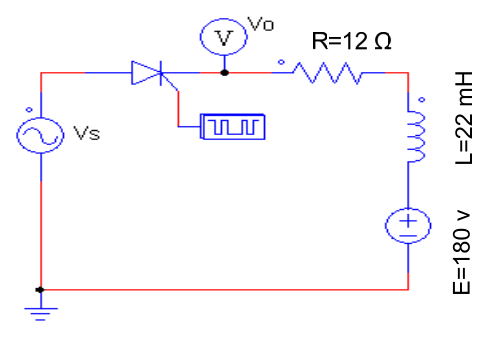
\includegraphics[scale=0.75]{./image/Screenshot22.png}\\
\caption{Circuito RLE tir\'{i}storizado}
\label{grafico 10}
\end{figure}\par
%2
\item
Considere $\alpha = 60º$\par
%
\begin{enumerate}
%2a
\item
Obtenha, socorrendo-se do {\bf Excel}, as formas de onda para as grandezas $I_o(\omega t)$, $V_s(\omega t)$, $V_o(\omega t)$, $V_R(\omega t)$ e $V_L(\omega t)$;\par
%
\begin{figure}[H]
\centering
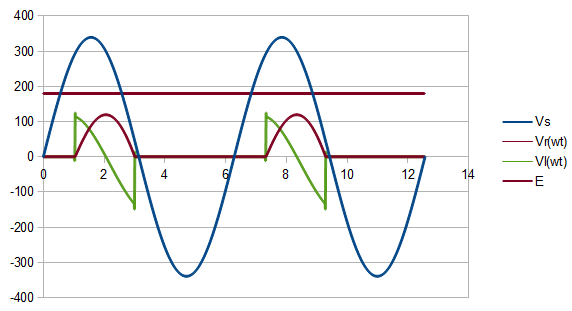
\includegraphics[width=0.90\linewidth]{./image/P2A2p2a_1.png}\\
\caption{Tens\~{o}es}
\label{grafico 11}
\end{figure}\par
%
\begin{figure}[H]
\centering
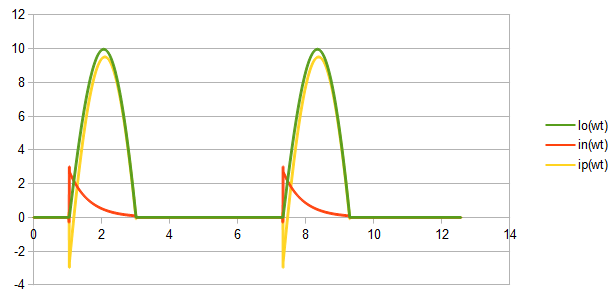
\includegraphics[width=0.90\linewidth]{./image/P2A2p2a_2.png}\\
\caption{Correntes}
\label{grafico 12}
\end{figure}\par
%2b
\item
Repita a al\'{i}nea b), mas com $\alpha = 90º$;\par
%
\begin{figure}[H]
\centering
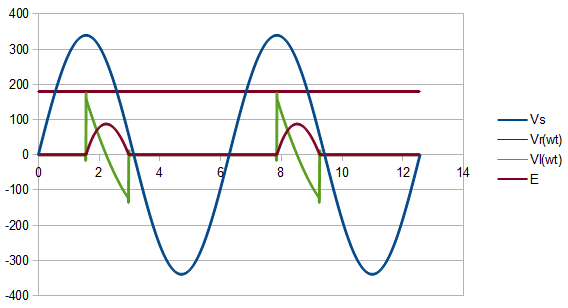
\includegraphics[width=0.90\linewidth]{./image/P2A2p2b_1.png}\\
\caption{Tens\~{o}es}
\label{grafico 13}
\end{figure}\par
%
\begin{figure}[H]
\centering
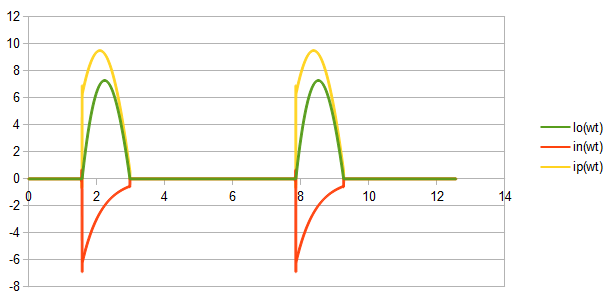
\includegraphics[width=0.90\linewidth]{./image/P2A2p2b_2.png}\\
\caption{Correntes}
\label{grafico 14}
\end{figure}\par
%2c
\item
Repita a al\'{i}nea b), mas com $\alpha = 120º$;\par
%
\begin{figure}[H]
\centering
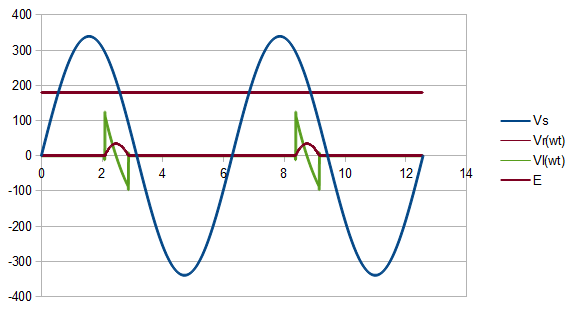
\includegraphics[width=0.90\linewidth]{./image/P2A2p2c_1.png}\\
\caption{Tens\~{o}es}
\label{grafico 15}
\end{figure}\par
%
\begin{figure}[H]
\centering
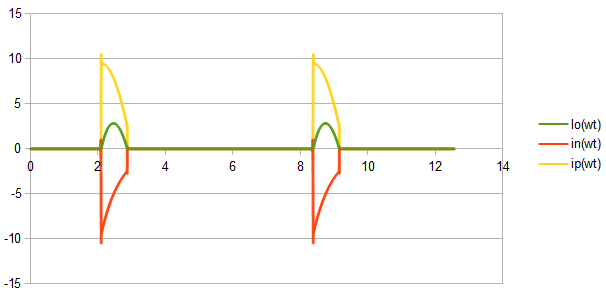
\includegraphics[width=0.90\linewidth]{./image/P2A2p2c_2.png}\\
\caption{Correntes}
\label{grafico 16}
\end{figure}\par
%2d
\item
Repita a al\'{i}nea b), mas com $\alpha = 30º$;\par
%
\begin{figure}[H]
\centering
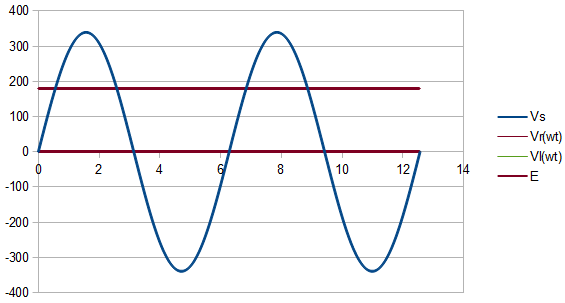
\includegraphics[width=0.90\linewidth]{./image/P2A2p2d_1.png}\\
\caption{Tens\~{o}es}
\label{grafico 17}
\end{figure}\par
%
\begin{figure}[H]
\centering
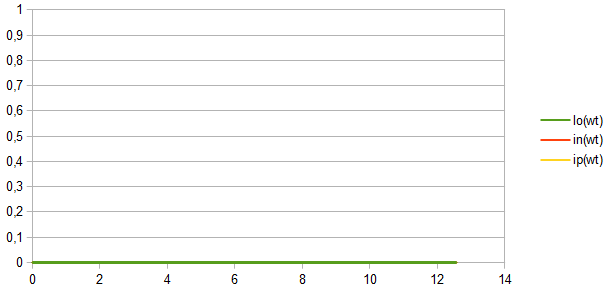
\includegraphics[width=0.90\linewidth]{./image/P2A2p2d_2.png}\\
\caption{Correntes}
\label{grafico 18}
\end{figure}\par
%
\end{enumerate}
%3
\item
Socorrendo-se do {\bf PSIM}*(3), obtenha as formas de onda para as mesmas grandezas e mesmos \^{a}ngulos $\alpha$, de disparo.\par
%
a)\par
%
\begin{figure}[H]
\centering
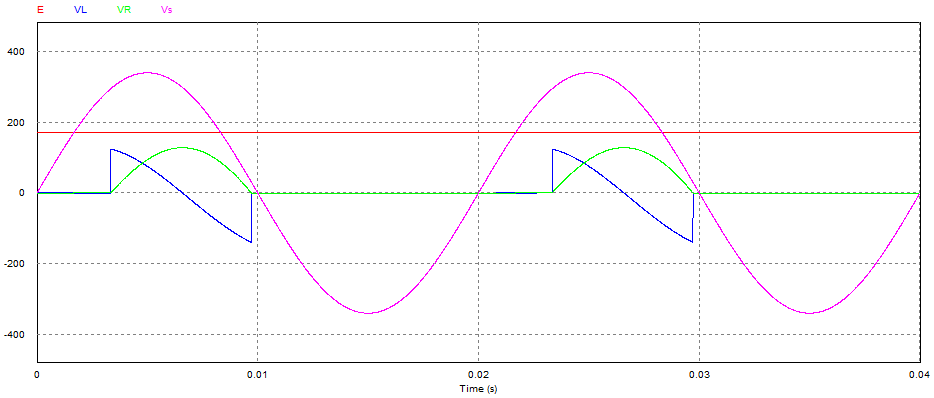
\includegraphics[width=0.90\linewidth]{./image/P2A2p3a_1.png}\\
\caption{Tens\~{o}es}
\label{grafico 19}
\end{figure}\par
%
\begin{figure}[H]
\centering
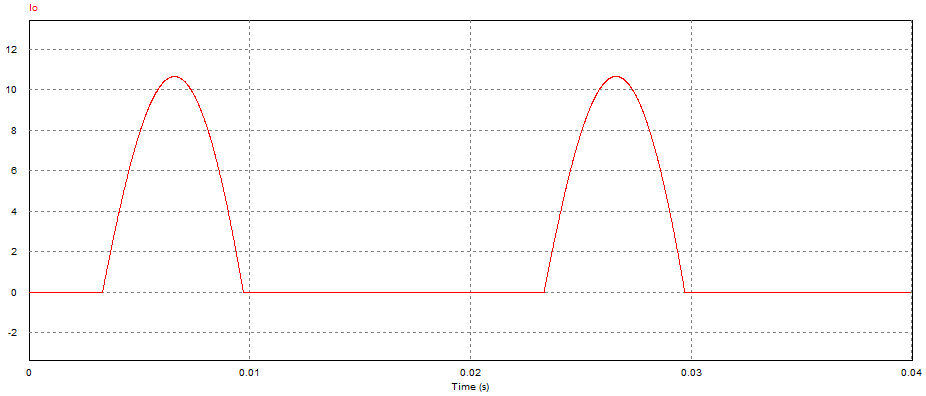
\includegraphics[width=0.90\linewidth]{./image/P2A2p3a_2.png}\\
\caption{Correntes}
\label{grafico 20}
\end{figure}\par
%
b)\par
%
\begin{figure}[H]
\centering
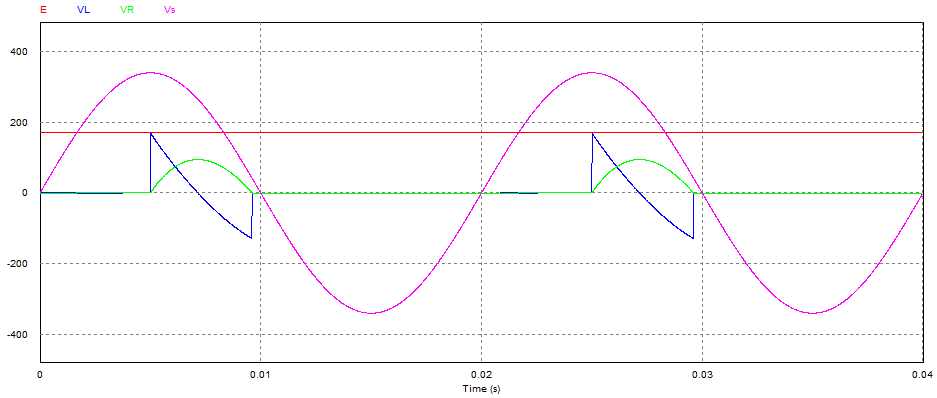
\includegraphics[width=0.90\linewidth]{./image/P2A2p3b_1.png}\\
\caption{Tens\~{o}es}
\label{grafico 21}
\end{figure}\par
%
\begin{figure}[H]
\centering
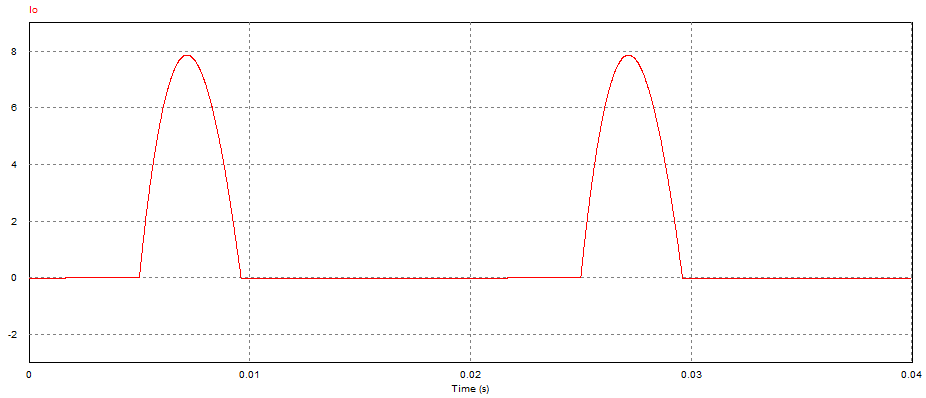
\includegraphics[width=0.90\linewidth]{./image/P2A2p3b_2.png}\\
\caption{Correntes}
\label{grafico 22}
\end{figure}\par
%
c)\par
%
\begin{figure}[H]
\centering
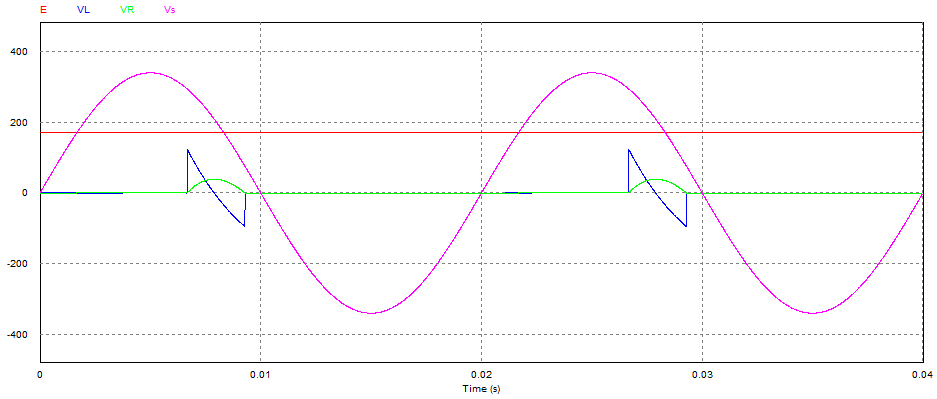
\includegraphics[width=0.90\linewidth]{./image/P2A2p3c_1.png}\\
\caption{Tens\~{o}es}
\label{grafico 23}
\end{figure}\par
%
\begin{figure}[H]
\centering
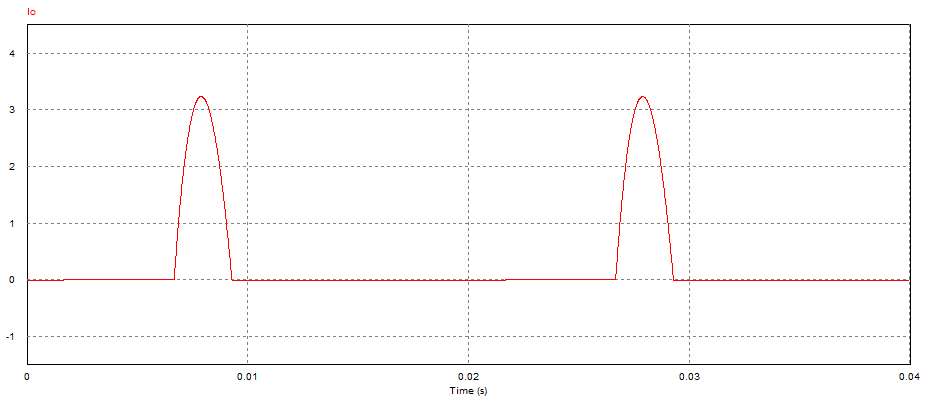
\includegraphics[width=0.90\linewidth]{./image/P2A2p3c_2.png}\\
\caption{Correntes}
\label{grafico 24}
\end{figure}\par
%
d)\par
%
\begin{figure}[H]
\centering
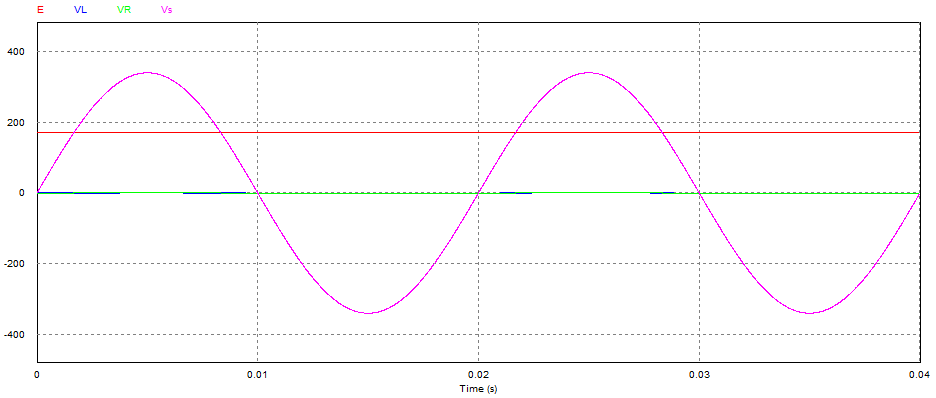
\includegraphics[width=0.90\linewidth]{./image/P2A2p3d_1.png}\\
\caption{Tens\~{o}es}
\label{grafico 25}
\end{figure}\par
%
\begin{figure}[H]
\centering
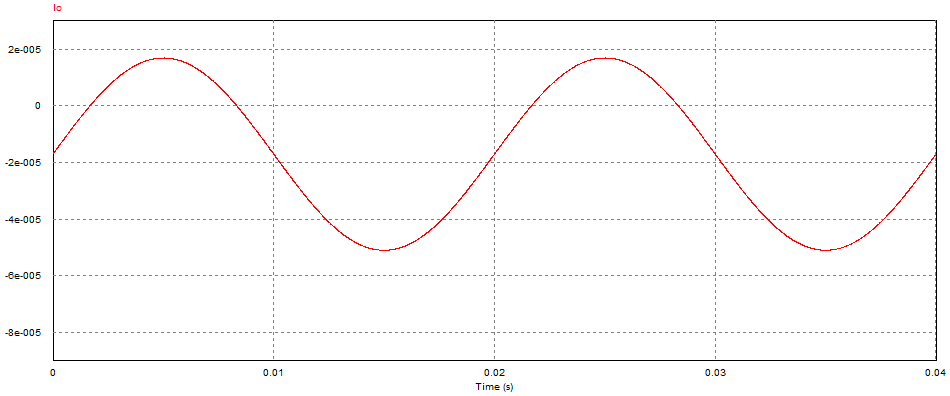
\includegraphics[width=0.90\linewidth]{./image/P2A2p3d_2.png}\\
\caption{Correntes}
\label{grafico 26}
\end{figure}\par
%
\end{enumerate}
%
\begin{itemize}
\item 
Para efeitos de simula\c{c}\~{a}o, utilize para disparo do tir\'{i}stor o elemento “Gating Block”, em que o impulso de disparo tem a dura\c{c}\~{a}o  de $1^o$. (Quanto vale $1^o$ em termos de tempo ?)\par
% 
\end{itemize}
%
\begin{abstract}
%
Nesta Parte \ref{P2A2} atrav\'{e}s do {\bf libreOffive} foi representado as formas de onda para diversos disparos do tir\'{i}stor, os resultados pela folha de calculo são pr\'{o}ximos dos adquiridos pelo simulador {\bf PSIM}.
O tir\'{i}stor tem que respeitar certos requisitos para funcionar, tal como a corrente tem que ser positiva de \^{A}nodo a Catodo, e os disparos tem que ocorrer quando a condi\c{c}\~{a}o inicial apresentar uma corrente positiva imediatamente ap\'{o}s o disparo.
No {\bf PSIM} a largura dos disparos podem ser definidos ao nosso crer.
%
\end{abstract}
%
%%%%%%%%%%%%%%%%%%%%%%%%%%%%%%%%%%%%%%%%%%%
%
\part{Equa\c{c}\~{o}es} \label{eq}
%
\begin{flushleft}
{\bf Corrente Continua Condi\c{c}\~{o}es \index{Condi\c{c}\~{o}es} iniciais \index{iniciais} nulas \index{nulas}.}\par
\end{flushleft}
 \quad Circuito \index{Circuito} $LC$ em $C.C$:\par
%
\begin{itemize}
\item
$i(t)=\frac{V_{DC}\sqrt{LC}}{L}\quad \sin \left( \frac{t}{\sqrt{LC}}\right)\times u(t)$\par
\item
$V_L(t)=V_{DC}\quad \cos\left(\frac{t}{\sqrt{LC}} \right)\times u(t)$\par
\item
$V_c(t)=V_{DC}\quad \left(1-\cos\left(\frac{t}{\sqrt{LC}} \right) \right)\times u(t)$\par
\item
$\omega_n=\frac{1}{\sqrt{LC}}$\par
\item
$\overline{Z}=\sqrt{(\omega_n L-\frac{1}{\omega_n C})^2}$\par
\item
$\phi_p=\frac{\pi}{2}$\par
porque, $\sin(\omega_n t)= \cos(\omega_n t - \pi/2)$\par
\item
$\tau=\infty$\par
\end{itemize}
%
%%%%%%%%%%%%%%%%%%%%%
\quad Circuito \index{Circuito} $RLC$ em $C.C$:\par
%
\begin{enumerate}
%enum1
\item
Para \quad $C(C R^2-4 L)>0$ \quad (Ra\'{i}zes \index{Ra\'{i}zes} reais \index{reais} diferentes \index{diferentes}) \quad Sobreamortecido \index{Sobreamortecido}.\par
%
\begin{itemize}
\item
$i(t)=\frac{2 V_{DC} C e^{\frac{-tR}{2L}} sinh \left( \frac{t \sqrt{C(CR^2-4L)}}{2CL} \right)}{\sqrt{C(CR^2-RL)}}\times u(t)$\par
\item
$V_R(t)=R\times i(t)$\par
\item
$V_L(t)=L\dfrac{di(t)}{dt}$\par
%
\begin{minipage}{0.95\linewidth}
\makebox[\linewidth]{
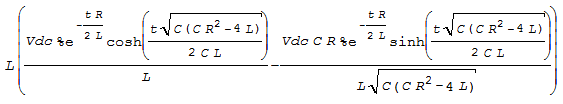
\includegraphics[scale=0.75]{./image/equacoes_1.png}
}
\end{minipage}\par
%
\item
$V_C(t)=\frac{1}{C}\int_0^ti(t)$\par
%
\begin{minipage}{0.95\linewidth}
\makebox[\linewidth]{
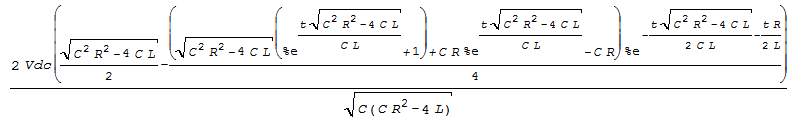
\includegraphics[scale=0.75]{./image/equacoes_2.png}
}
\end{minipage}\par
%
\end{itemize}
%enum2
\item
Para \quad $C(C R^2-4 L)=0$ \quad (Ra\'{i}zes \index{Ra\'{i}zes} iguais \index{iguais})\quad Amortecimento \index{Amortecimento} cr\'{i}tico \index{cr\'{i}tico}.\par
%
\begin{itemize}
\item
$i(t)=\frac{V_{DC}}{L} \quad  t \quad e^{\frac{-R t}{2L}} \times u(t)$\par
\item
$V_R(t)=R\times i(t)$\par
\item
$V_L(t)=L\dfrac{di(t)}{dt}$\par
%
\begin{minipage}{0.95\linewidth}
\makebox[\linewidth]{
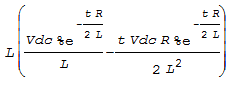
\includegraphics[scale=0.75]{./image/equacoes_3.png}
}
\end{minipage}\par
%
\item
$V_C(t)=\frac{1}{C}\int_0^ti(t)$\par
\begin{minipage}{0.95\linewidth}
\makebox[\linewidth]{
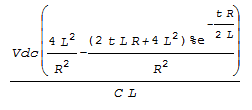
\includegraphics[scale=0.75]{./image/equacoes_4.png}
}
\end{minipage}\par
%
\end{itemize}
%enum3
\item
Para \quad $C(C R^2-4 L)<0$ \quad (Ra\'{i}zes \index{Ra\'{i}zes} complexas \index{complexas}) \quad Amortecido \index{Amortecido}.\par
%
\begin{itemize}
\item
$i(t)=\frac{2 V_{DC} C e^{\frac{-tR}{2L}} sin \left( \frac{t \sqrt{-C(CR^2-4L)}}{2CL} \right)}{\sqrt{-C(CR^2-4L)}}\times u(t)$\par
\item
$V_R(t)=R\times i(t)$\par
\item
$V_L(t)=L\dfrac{di(t)}{dt}$\par
%
\begin{minipage}{0.95\linewidth}
\makebox[\linewidth]{
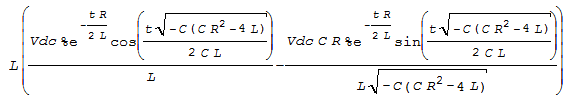
\includegraphics[scale=0.75]{./image/equacoes_5.png}
}
\end{minipage}\par
%
\item
$V_C(t)=\frac{1}{C}\int_0^ti(t)$\par
%
\begin{minipage}{0.95\linewidth}
\makebox[\linewidth]{
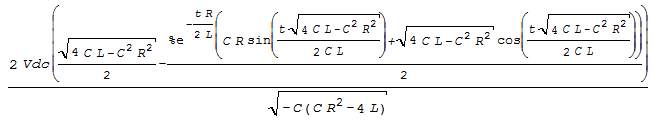
\includegraphics[scale=0.75]{./image/equacoes_6.png}
}
\end{minipage}\par
%
\end{itemize}
\end{enumerate}
%
\begin{itemize}
\item
$| \omega_n |=\sqrt{\frac{4 L-R^2 C}{4 L^2 C}}$\par
\item
%\overrightarrow{Z}
$\overline{Z}=\sqrt{R^2 + (\omega_n L -\frac{1}{\omega_n C})^2}$\par
\item
$\phi_p=\arctan\left(\frac{\omega_n L - \frac{1}{\omega_n C}}{R}\right)$\par
\item
$\tau=\frac{2 L}{R}$\par
\end{itemize}
%%%%%%%%%%%%%%%%%%%%%%%%%%%%%%%%%%%%%%%%%%
\begin{flushleft}
{\bf Corrente \index{Corrente} Alternada condi\c{c}\~{o}es \index{Condi\c{c}\~{o}es} iniciais \index{iniciais} nulas \index{nulas}}.
\end{flushleft}
\quad Circuito \index{Circuito} $RLE$ em $C.A$:\par
\begin{itemize}
\item
$i(t)=C_T\ e^{-\frac{R}{L}t}+\frac{V_{m\acute{a}x}}{\overline{Z}}\sin(\omega t + \alpha - \phi_p)-\frac{E}{R}$\newline
$i(t)=C_T\ e^{-\frac{R}{L}t} + C_1 \cos (\omega t) + C_2 \sin(\omega t)-\frac{E}{R}$
\item
$I(\omega t)=C_T\ e^{-\frac{R}{L \omega}\omega t}+\frac{V_{m\acute{a}x}}{\overline{Z}}\sin(\omega t + \alpha - \phi_p)-\frac{E}{R}$
\item
$\overrightarrow{Z}=R+j\omega L$\\
$\overline{Z}=\sqrt{R^2 + (\omega L)^2}$
\item
$\phi_p=\arctan(\frac{\omega L}{R})$
\item
$C_T=\frac{E}{R}-\frac{V_{m\acute{a}x}}{\overline{Z}}\sin(\alpha - \phi_p)$
\item
$C_T=\frac{V_{m\acute{a}x}}{R^2 + (\omega L)^2}(L \omega \cos(\alpha) - R \sin (\alpha))+\frac{E}{R}$
\item
$C_1=\frac{V_{m\acute{a}x}}{R^2 + (\omega L)^2}(R \sin (\alpha) - L \omega \cos(\alpha))$
\item
$C_2=\frac{V_{m\acute{a}x}}{R^2 + (\omega L)^2}(R \cos (\alpha) + L \omega \sin (\alpha))$
%
\end{itemize}
%%%%%%%%%%%%%%%%%%%%%%%%%%%%%%%%%%
\begin{definition}
Capacit\^{a}ncia
\begin{flalign*}
Q_c(t) =& \int^t i(t) \quad dt & \\
=& Q_c(0^-)+\int_{0^-}^t i(t) \quad dt & \\
V_c(t) =& \frac{Q_c(t)}{C} & \\
=& \frac{1}{C} \quad \int^t i_c(t) \quad dt & \\
=& \frac{Q_c(0^-)}{C} + \frac{1}{c} \quad \int_0^t i_c(t) \quad dt & \\
=& V(0^-) + \frac{1}{c} \quad \int_0^t i_c(t) \quad dt & \\
i_c(t) =& C \quad \dfrac{d V_c(t)}{dt} &
\end{flalign*}\par
\end{definition}
%
\begin{definition}
Indut\^{a}ncia
\begin{flalign*}
\psi_L(t) =& \int^t V_L(t) \quad dt & \\
=& \psi_L(0^-)+\int_{0^-}^t V_L(t) \quad dt & \\
V_L(t) =& L \quad \dfrac{d i_L(t)}{dt} & \\
i_L(t) =& \frac{\psi_L(t)}{L} & \\
=& \frac{1}{L} \quad \int^t V_L(t) \quad dt & \\
=& \frac{\psi_L(0^-)}{L} + \frac{1}{L} \quad \int_0^t V_L(t) \quad dt & \\
=& i_L(0^-) + \frac{1}{L} \quad \int_0^t V_L(t) \quad dt &
\end{flalign*}\par
\end{definition}
%
\begin{definition}
Resist\^{e}ncia
\begin{flalign*}
V_R(t) =& R \quad i_R(t) & \\
i_R(t) =& \frac{V_R(t)}{R} &
\end{flalign*}\par
\end{definition}
%
\begin{definition}
Valor M\'{e}dio
\begin{flalign*}
X_{av} =& \frac{1}{T} \; \int_0^T X(t) dt &
\end{flalign*}\par
\end{definition}
%
\begin{definition}
Valor Eficaz
\begin{flalign*}
X_{ef} =& \sqrt{ \frac{1}{T} \; \int_0^T \overset{\text{2}}{X(t)} dt } &
\end{flalign*}\par
\end{definition}
%

%
%%%%%%%%%%%%%%%%%%%%%%%%%%%%%%%%%%%%%%%%%%%
\newpage
\listoffigures
\cite{*}
\bibliography{./bibliography/Bibliography}
%\printindex
\newpage
\footnote{Apontamentos Electr\'{o}nica de Pot\^{e}ncia}
%
\end{document}
